
\section{Motivation}

As a software engineers,
we often came across software destributed
in a form of docker containers alongside
of traditional binary files,
or articles comparing docker to the other kind of virtualization techniques,
or DevOps research papers comparing the performance of cloud instances in AWS,
but did not know what it was about.
Main goal of this research for us is to provide an answer
for an important question, whether it is worth
to change our infrastructures
from virtualized hardware to Docker, or stick to KVM, for example.

Virtualization was invented long before mid-2000s,
but has only became mainstream for the industry at the
time of its invention in the mid-2000.
Smart virtualization engines such as Linux-based QEMU, KVM, Xen
and their Windows-based rival Hyper-V changed the IT industry forever,
sufficiently decreasing the need for dedicated and local hardware.

This shift has made a cloud computing from abstract theory to the reality,
creating huge benefits for cloud providers like Amazon AWS,
Microsoft Azure and Google.
However, the virtualization was not perfect, as any advanced technology:
as obvious as their advantages were, it had many drawbacks mainly in maintenance
of the complicated virtualized infrastructure.

With the first release of its state-of-the-art Docker library for Linux,
developer Solomon Hikes provided its own way of solving these problems,
which has not only became successful startup
with capitalization of over two billions USD as of October 2017,
but also a major breakthrough in the IT Field, almost pushing the existing
businesses and startups in maintaining advanced virtualized infrastructure
to the edge of survival or even completely eliminating
them from the market for good.

\section{Long way to Docker}

Some technologies evolved itself from the existing ideas
or approach at the time of invention, and Docker is no exclusion.
The aim of this section is to provide an overview of main competitive
technologies referenced as industry standardards
before the era of Docker, their advantages and disadvantages.

\subsection{Server architecture without virtualization}

A traditional server is just a hardware unit
which has an operating system installed,
which then supervises applications running.

\begin{figure}
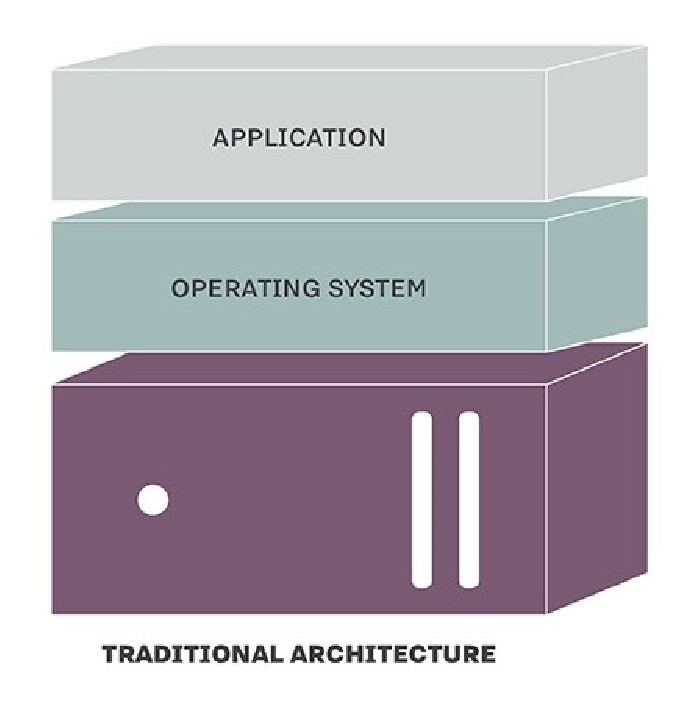
\includegraphics[height=3in, width=3in]{traditional}
\caption{Principal scheme of Data center architecture without virtualization}
\cite{TraditionalAndVirtualInfra}
\end{figure}

Though perfectly well suitable for normal user, this architecture
has proven itself as unreliable, non-scalable,
and generally not suitable for long-term enterprise environments support.

The operating system layer was usually installed manually or with
installation scripts specially written for that purpose,
and the enterprise application running inside these
environments were configured from within the OS by the system administrators.

\subsection{Virtualization}

\subsubsection{Invention and definition}

At the beginning of computer era, in the year of 1964,
computer architecture, both its hardware and software
parts allowed simultaneous execution of instructions only from only one user
currently active in a system. It was not suitable for the customers, however.
The research team got a grant from DARPA, and
rolled out its first virtualization solutions based on a time-sharing,
and later also on memory-sharing.

\begin{definition}
Virtualization is a technology of clear and safe dividing
of existing hardware resources amongst the "host" operating system,
which has a direct access to the hardware resources and where the
virtualization program is started, and some of the "guest" operating systems,
which lifecycle is maintained and supervised by the abovementioned software.
\end{definition}

With the invention of the virtualization first as software solution,
it has become possible for one server to serve multiple users at a time
significantly decreasing stall times and the need for excessive hardware.
Moreover, it became possible to sell the unused
server power to the other commercial entities or private customers,
bringing additional profit to the organization.

Even after its invention, it was inaccessible
for the industry mainly because of

\subsubsection{Binary virtualization}







\begin{figure}
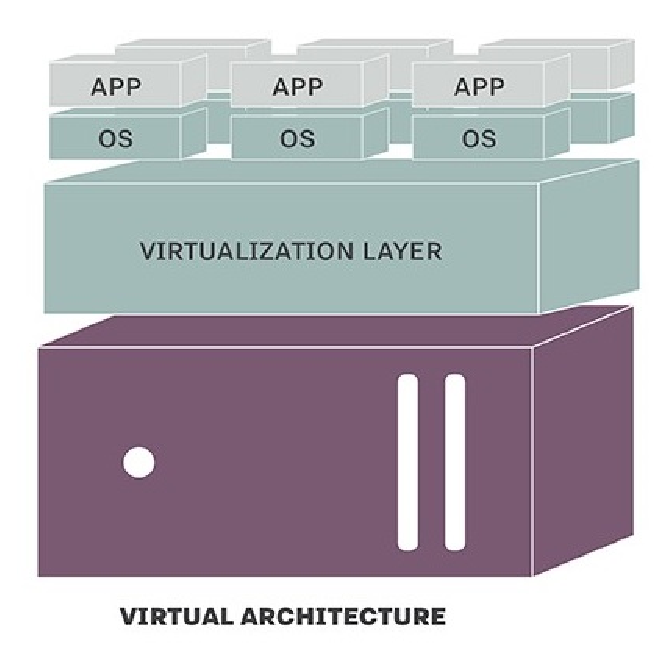
\includegraphics[height=3in, width=3in]{virtualized}
\caption{Principal scheme of virtualized infrastructure}
\cite{TraditionalAndVirtualInfra}
\end{figure}

\subsection{Paravirtualization}

First implemented and desciribed by Xen Project,

\begin{definition}
Paravirtualization (PV) is an efficient and lightweight virtualization technique
introduced by the Xen Project team, later adopted by other
virtualization solutions. PV does not require virtualization extensions from
the host CPU and thus enables virtualization on hardware architectures that do
not support Hardware-assisted virtualization.
However, PV guests and control domains require kernel
support and drivers that in the past required special kernel builds,
but are now part of the Linux kernel as well as other operating systems.\cite{ParavirtualizationDefinition}
\end{definition}

\begin{figure}
\includegraphics[height=3in, width=3in]{paravirtualized}
\caption{Principal scheme of paravirtualization initially made by Xen project}
\end{figure}

\subsubsection{Hardware-assisted virtualization}

With growing demand of personal customers and commercial entities

\subsection{Unsolved problems of the virtualization}


With the brilliance of these technologies as it is,
some of the problems never found it solutions completely:
First of all, all of the virtual systems
need to be updated regularly, not only for the obvious reason of security,
but also for the sake of prolonged maintaining of deployed applications.
Second, all the virtualized infrastructure had the
need to be backed up regularly to
prevent the loss of important business information.
With the complexity of the infrastructures
growing exponentially, the need for additional
employments made an impact on the industry

\section{Docker principles}

In 2010, individual developer Solomon Hikes came up with an idea that was
supposed to provide an answer to all of the challenges brought up by different
virtualization techniques: instead of virtualizing hardware resources running
several operating systems at the same time, it would have been possible
to launch only one instance of OS and spare not only storage and memory capacity,
but also a CPU operations by performing all
OS activities (like rescheduling) only once, which should theoretically
improve performance
The goal of this chapter is to provide detailed overview of Docker architecture
and the ways it does perform its tasks.

\subsection{Container}

As stated by the Docker Inc., the inventor of Docker technology,

\begin{definition}
A container image is a lightweight, stand-alone,
executable package of a piece of software that includes everything
needed to run it: code, runtime,
system tools, system libraries, settings. \cite{DockerDefinition}
\end{definition}

Container is another type of virtualization approach.
Containers and virtual machines have
similar resource isolation and allocation benefits,
but function differently because containers
virtualize the operating system instead of hardware.
Containers are more portable and efficient,
as can be seen on the picture 3.

\subsection{Docker architecture}

Docker is a software product consisting mainly of a
library written in Go programming language
which acts as an intermediary between apps packaged
in the container and the Linux kernel.

\begin{figure}
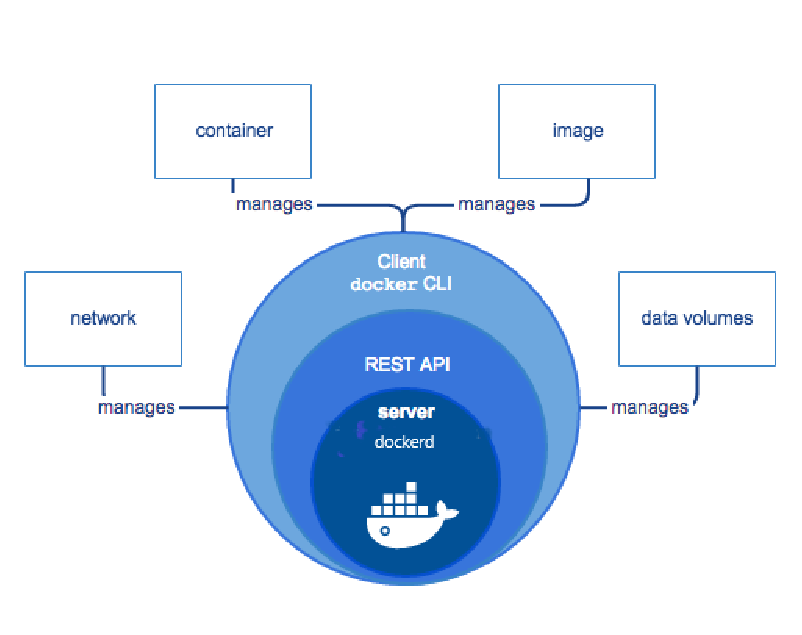
\includegraphics[height=3in, width=3in]{dockerarch}
\caption{Scheme of Docker architecture}
\end{figure}

Without following advanced Linux kernel features,
the development of Docker would not have been possible:

control groups (named cgroups for the sake of simplicity) is
Linux kernel feature which allows it to restrict
each application to the specific set of resources, or allocate resources —
such as CPU time, system memory, network bandwidth,
or combinations of these resources — among user-defined groups
of tasks (processes) running on a system.\cite{CGroupsDefinition}

SELinux - a special kernel extension, which adds advanced security features to
the OS, mainly fine-grained file control, but can also be applied
for the interprocess communication and network resources. \cite{SELinuxDef}
This is one of the feature of the kernel, which has utter importance for Docker,
because without it would not have been possible to isolate files or ports
of the containers from the other containers trying to access this files,
which in turn would have led to security issues.
Docker employees have even described their software as being "Secure By Default"
in their blog post \cite{SELinuxDockBlog}

namespaces -

Netlink -

AppArmor -

capabilities -

Moreover, the docker library is able to determine when multiple container
applications share the same libraries
and provide it for them at the time needed.
That way
The main advantage of Docker is that it uses already existing features
provided by the Linux operating system.

\subsubsection{Docker Image}

To use docker, a docker image ought to be created.
An image is compiled by docker engine itself,
using a script file provided by user called Dockerfile.
One of the most powerful features of docker is inheritance,
 so usual approach in the industry
is to create a base image and extend it with
new features later when there is such a necessity.
A base image is extended using FROM directive like this:
FROM: ubuntu 16.10
Using the RUN directive, different commands supported by the base operating
system can be passed to the container for setting up the image like this:
RUN sudo apt-get install mariadb
Moreover, the files needed by the applications can be copied directly
into the image using the COPY directive:

\subsubsection{Using a container}

Once an image is created, it can be deployed into a container. A
container in terms of docker is nothing more than a running
instance of Host OS, where the docker is installed. It can be placed
in the cloud or on the local hardware.
Created containers can be launched, stopped, and queried for their
current state for maintenance work at will, exactly like normal virtual
machine can be. Upon container creation it is possible to pass
different launch parametres like an automatic restart if the server
has been turned off by some reason.

\subsubsection{Union file system}

While proven to reduce average CPU load and memory usage by
eliminating the redundant duplication of the OS components of the
virtual environments,
unionfs (Union File System, further referred as UFS), a file system
initially developed by and further maintained by the open source
community, is one of the most crucial parts of docker system.
UFS consits of “layers”, abstract file system units clearly separated
from each other, with some of them write-protected. This allows
docker core to maintain one and the only copy of the operating
system files necessary for its working declaring it unchangeable
while keeping the changeable files belonging to different images
unreachable from within other layers thus making it impossible to
alter or delete them, drastically improving the security of the virtual
environments.

\subsubsection{Container registry}

As stated before in the chapter 3.1, docker image consists of multiple layers.
It is supposed to be convenient for the end user,
but has a fundamental problem: if we have
n images based on some kind of operating system, and we need
to distribute it to m servers, the OS image itself will be downloaded
n x m times, which leads to increased
load on the docker CDN \footnote{Content delivery network}

But Docker engineers have found a way to solve this problem by providing
a special service called Docker registry. It is a special service for uploading
custom images or its updates in a way, that only the necessary layers will be
downloaded by the consumers.

Docker Registry is provided by docker incorporation and is available
as a free public service or open-source software
for the installation on the own infrastructure.
That way the commercial entities, developer teams or even individuals having a
wish to hide their images from the public access
are not bound to the usage of Docker Inc. as their unique provider, that means
no vendor lock is present.

\subsubsection{Container interaction}

In case when there is more than one container
instance running on the docker server, it can become increasingly difficult for
to users to maintain them.

\section{Orchestration}

\subsection{Native ecosystem}

\subsubsection{Docker Machine}

\subsubsection{Docker Swarm}

\subsubsection{Docker Compose}

\subsection{Kubernetes}

\section{Conclusions}

As a result of this research work, it became clear to us that, first of all,
the approach of container virtualization or containerization
is the future of software deployment, because it not only reduces complexity of
different types of infrastructure like content delivery network,
but also significantly reduces server load, significantly
increases security of the deployed application,
because the possibly infected software cannot
escape its file system layer and has no direct access
to the operating system where the docker process is running, and is
especially usable for shipping software images to the different types of customers,
from the most inexperienced ones to hardcore professionals.

The approach has drawbacks, too, mainly
because it is relatively new to the market,
and it is pretty hard for industry to find
a sufficient amount of system administrators or special
administering software qualified to support advanced docker infrastructures.



\appendix
%Appendix A
\section{Headings in Appendices}
The rules about hierarchical headings discussed above for
the body of the article are different in the appendices.
In the \textbf{appendix} environment, the command
\textbf{section} is used to
indicate the start of each Appendix, with alphabetic order
designation (i.e., the first is A, the second B, etc.) and
a title (if you include one).  So, if you need
hierarchical structure
\textit{within} an Appendix, start with \textbf{subsection} as the
highest level. Here is an outline of the body of this
document in Appendix-appropriate form:
\subsection{Introduction}
\subsection{The Body of the Paper}
\subsubsection{Type Changes and  Special Characters}
\subsubsection{Math Equations}
\paragraph{Inline (In-text) Equations}
\paragraph{Display Equations}
\subsubsection{Citations}
\subsubsection{Tables}
\subsubsection{Figures}
\subsubsection{Theorem-like Constructs}
\subsubsection*{A Caveat for the \TeX\ Expert}
\subsection{Conclusions}
\subsection{References}
Generated by bibtex from your \texttt{.bib} file.  Run latex,
then bibtex, then latex twice (to resolve references)
to create the \texttt{.bbl} file.  Insert that \texttt{.bbl}
file into the \texttt{.tex} source file and comment out
the command \texttt{{\char'134}thebibliography}.
% This next section command marks the start of

\begin{acks}
  The authors would like to thank Dr. Yuhua Li for providing the
  MATLAB code of the \textit{BEPS} method.

  The authors would also like to thank the anonymous referees for
  their valuable comments and helpful suggestions. The work is
  supported by the \grantsponsor{GS501100001809}{National Natural
    Science Foundation of
    China}{http://dx.doi.org/10.13039/501100001809} under Grant
  No.:~\grantnum{GS501100001809}{61273304}
  and~\grantnum[http://www.nnsf.cn/youngscientists]{GS501100001809}{Young
    Scientists' Support Program}.

\end{acks}
